\textit{Programmable Logic Controller} (\gls{plc}) je vestavěný počítač, který
zpracovává vstupy, provádí jejich vyhodnocování, komunikuje s~dalšími \gls{plc}
obvody a~nastavuje výstupy \cite{plc:web}. Na rozdíl od běžných počítačů typu
\textit{PC} mají \gls{plc} větší množství vstupů a~výstupů, běží na nich
\textit{realtime} operační systémy a~jsou vysoce robustní.

\gls{plc} jsou základní jednotkou průmyslové automatizace. Používají se
například pro řízení světel dopravních křižovatek, výrobních linek, eskálátorů,
řízení elektráren, rozvoden apod. Všude tam \gls{plc} zpracovávají data z~čidel
a~ovládají periferie – například motorické pohony, signalizační diody,
robotické ruky, lasery apod.

\begin{figure}[ht]
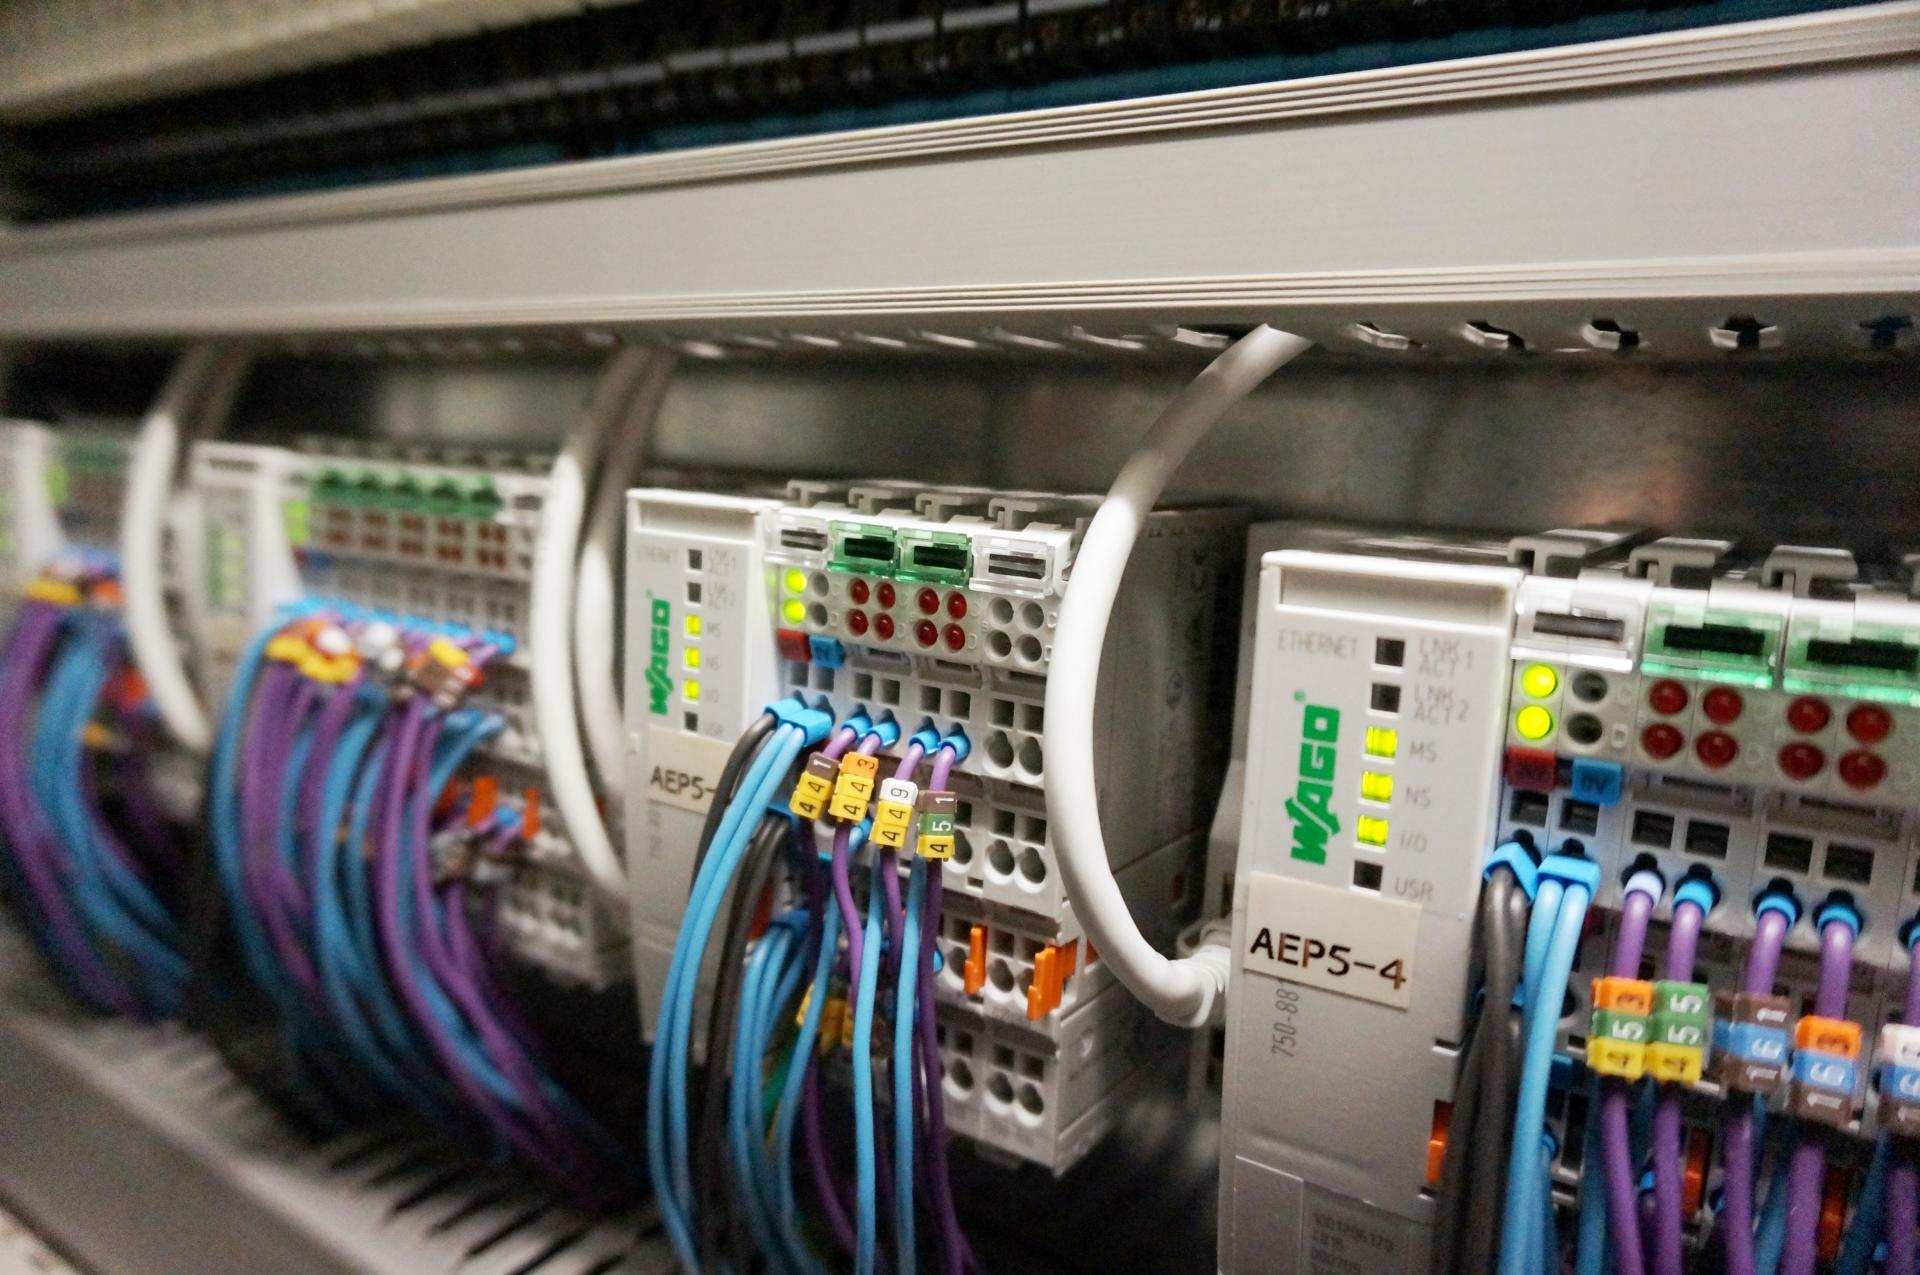
\includegraphics[width=0.7\textwidth]{data/plc.jpg}
\caption{Průmyslové \gls{plc} moduly. Převzato z~\texttt{wikimedia.org}.}
\label{fig:mtbusb-prototype}
\end{figure}

V~této práci se zaměříme na podmnožinu \gls{plc} modulů – totiž na takové,
jejichž hlavním úkolem je správně zpracovávat vstupní signály a~ovládat výstupní
periferie. Řízení logiky průmyslového procesu přenecháme počítači, s~kterým
\gls{plc} moduly komunikují.\footnote{V~praxi může \gls{plc} modul řídit logiku
procesu přímo, my však tuto situaci zkoumat nebudeme.}

Cílem této práce je navrhnout a~implementovat novou verzi komunikační sběrnice
\gls{plc} obvodů zvanou \textit{\gls{mtbbus}} (\textit{Model Train
Bus}\footnote{Expanze zkratky do jejího plného významu nedává smysl, i~tak
budeme používat označení MTBbus, protože tak je zkratka zaužívaná.}).

\gls{mtbbus} je sběrnice, která se využívá pro řízení modelových kolejišť.
Je součástí systému \gls{mtb}. Skrze sběrnici lze číst signály z~kolejiště
(například polohy výhybek, obsazenost kolejových obvodů) a~povelovat prvky
v~kolejišti (návěstidla, přestavníky výhybek, přejezdy apod.). Obdobným
způsobem funguje zapezpečovací zařízení na skutečné železnici.

V~této práci autor nejprve popíše současné nasazení systému \gls{mtb}. Budou
formulovány důvody vedoucí k~nutnosti aktualizace sběrnice. Autor popíše, proč
jsou dostupná komerční řešení nevhodná a~navrhne vlastní nové (1) protokoly,
(2) hardwarové moduly a~(3) počítačové programy, které jím formulovaný problém
řeší.
